
%・プレゼンター1人,傍聴者3人によるプレゼンテーションを行った

%・プレゼンと質問時間合わせて10分程度

%・提案アプリケーション+OEB使用時と,Zoomのみを使用した場合の2度行った

%・プレゼンター負担削減のため,プレゼン資料は事前に作成した(2種類)

%・また,各傍聴者に,最低一回の質問機会を設けるため,各プレゼンに対し3つの質問項目を事前に用意した

%・実験環境は以下の通り

%・共通:THETA VとTHETA Sを使用,プレゼンターは全天球カメラに対し30cmほど離れていた,プレゼンターのPC詳細(後で調べる)

%・Zoom使用時:質問者側はMac book pro(栗岡机上:後で詳しく)を使用(横に3人並んで一つの画面を見た)

%・OEB使用時:質問者側はOmniEyeBallを使用

プレゼンター1人,傍聴者3人によるプレゼンテーション実験を行った.

プレゼンテーション,及び質疑応答の時間合わせて10分程度の時間を設けた.

従来の平面ディスプレイでの表示を用いた実験,及び5-2節で説明したアプリケーション
を用いた実験の2通りを行った.本来はカウンターバランスをとるため,逆順で2回行う予定だったが,
コロナ感染対策のため参加人数を最小限に抑える必要があり,今回は1回での実験となった.

プレゼンターの負担の削減のため,プレゼンテーションのための資料は事前に作成した.
2通りの実験のため,2種類の資料が存在する.プレゼンテーションの内容は,
SNS用の宣材写真として東京工業大学の敷地内で何を写真に撮るのか,という題で
本館,または図書館を紹介するという物であった.

\begin{figure}[tp]
  \centering
  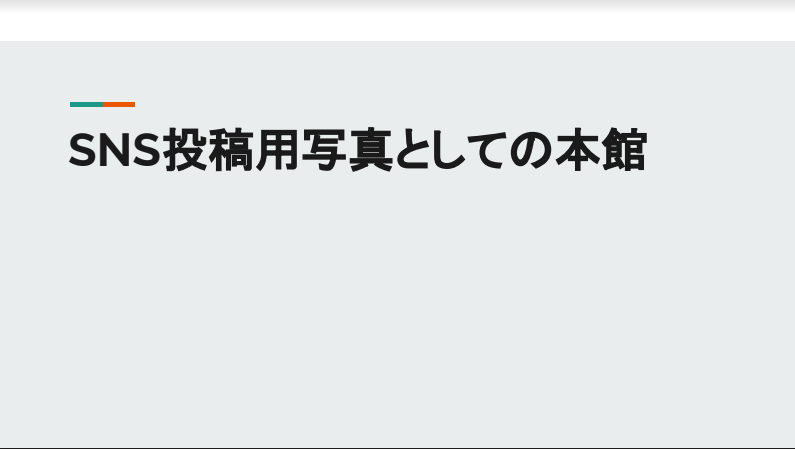
\includegraphics[scale=0.7]{fig/slide1.png}
  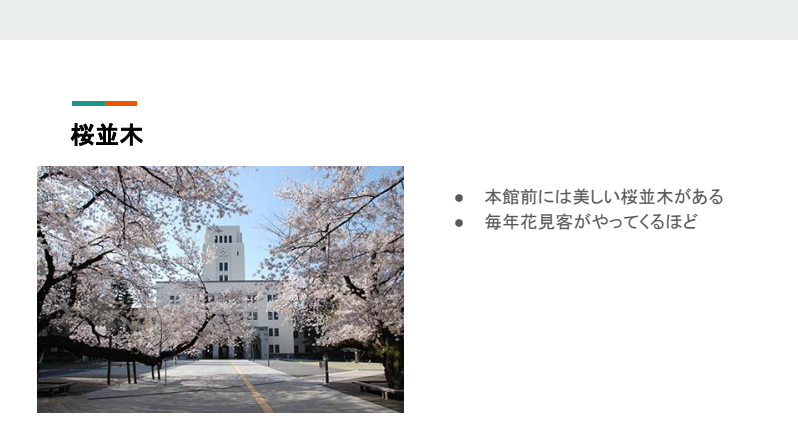
\includegraphics[scale=0.7]{fig/slide2.png}
  \caption{プレゼンターに用意したスライドの一部}
\end{figure}

また,各傍聴者には,それぞれ最低1回の質問機会を設けるため,各プレゼンテーション
に対して3つの質問項目を事前に用意した.

実験環境は以下の通りであった.

\begin{itemize}
  \item プレゼンターの全天球カメラとしてTHETA S,傍聴者側にはTHETA Vを用いた
  \item プレゼンターと傍聴者は全天球カメラからそれぞれ約40cm,50cmほど離れていた
  \item (プレゼンターと傍聴者側で用いたPCの詳細を後で書く)
  \item 傍聴者は平面ディスプレイを使用する際は,PCの前に設置した全天周カメラの前で横に並んで座っていた
  \item また,OmniEyeBallを使用する際は,120°の間隔で,球状ディスプレイを囲んで座っていた
\end{itemize}


